\documentclass[12pt,aspectratio=169]{beamer}
\usetheme{Berlin}
\usecolortheme{dolphin}
\beamertemplatenavigationsymbolsempty % remove navigation bar
%\setbeamercovered{transparent} % see future slides transparent

% Define a custom footline template
\setbeamercolor{title in head/foot}{bg=white, fg=gray}
\setbeamercolor{author in head/foot}{bg=white, fg=gray}
\setbeamercolor{date in head/foot}{bg=white, fg=gray}
\defbeamertemplate*{footline}{custom}{
  \leavevmode
  \hbox{
    \begin{beamercolorbox}[wd=0.5\paperwidth,ht=2.25ex,dp=1ex,center]{title in head/foot}%
      \usebeamerfont{title in head/foot}\insertshorttitle
    \end{beamercolorbox}
    \begin{beamercolorbox}[wd=0.2\paperwidth,ht=2.25ex,dp=1ex,center]{author in head/foot}%
      \usebeamerfont{author in head/foot}\insertshortauthor
    \end{beamercolorbox}
    \begin{beamercolorbox}[wd=0.2\paperwidth,ht=2.25ex,dp=1ex,center]{date in head/foot}
      \usebeamerfont{date in head/foot}\insertframenumber/\inserttotalframenumber
    \end{beamercolorbox}
  }
  \vskip0pt
}

% Create Title Card for each section
%\AtBeginSection[]{
%  \begin{frame}
%  \vfill
%  \centering
%  \begin{beamercolorbox}[sep=8pt,center,shadow=true,rounded=true]{title}
%    \usebeamerfont{title}\insertsectionhead\par%
%  \end{beamercolorbox}
%  \vfill
%  \end{frame}
%}

\usepackage[style=authoryear-icomp,maxbibnames=9,maxcitenames=2,backend=biber,sorting=nty,ibidtracker=false]{biblatex}
\setlength\bibitemsep{\baselineskip}
\usepackage[inkscapeformat=png]{svg}
\usepackage{ulem}
\usepackage{lmodern}
\usepackage{mathtools}
\usepackage{graphicx}
\usepackage[utf8]{inputenc}
\usepackage[T1]{fontenc}
\usepackage[english]{babel}
\usepackage{multicol}
\usepackage{animate}
\usepackage{tikz}
\usetikzlibrary{svg.path}
\usepackage{algorithm}% http://ctan.org/pkg/algorithm
\usepackage[noend]{algpseudocode}% http://ctan.org/pkg/algorithmicx
%\usepackage[hidelinks]{hyperref}
\usepackage{cleveref}
\usepackage{soul}
\usepackage{tcolorbox}
\usepackage{pifont}% http://ctan.org/pkg/pifont

\newcommand{\cmark}{\ding{51}}%
\newcommand{\xmark}{\ding{55}}%

\renewcommand*{\bibfont}{\normalfont\tiny}

%--------------------------------------------
% ALGORITHM CUSTOM BLOCKS
%--------------------------------------------
\renewcommand{\algorithmiccomment}[1]{{\color{gray}\hfill$//$\textit{#1}}} % Style for code comments

\newcounter{oldalglno} % allow parts of code without line numbering
\newenvironment{suppresslines}{\renewcommand\alglinenumber[1]{}\setcounter{oldalglno}{\value{ALG@line}}}{\setcounter{ALG@line}{\numexpr\value{oldalglno}\relax}}

\algrenewcommand\alglinenumber[1]{\tiny #1:} % make line numbers in code small

\algblock{Input}{EndInput}
\algnotext{EndInput}
\algblock{Output}{EndOutput}
\algnotext{EndOutput}
\newcommand{\Desc}[2]{\State {\boldmath\bfseries#1}\quad #2}

%--------------------------------------------
% MATH OPERATORS
%--------------------------------------------
\newcommand{\inv}[1]{#1^{-1}}
\newcommand{\convexhull}[1]{\text{conv}(#1)}

\DeclarePairedDelimiter{\ceil}{\lceil}{\rceil}
\DeclarePairedDelimiter{\floor}{\lfloor}{\rfloor}

\DeclareMathOperator*{\argmax}{arg\,max}
\DeclareMathOperator*{\argmin}{arg\,min}

% Make a space after every comma
\AtBeginDocument{%
  \mathchardef\stdcomma=\mathcode`,
  \mathcode`,="8000
}
\begingroup\lccode`~=`, \lowercase{\endgroup\def~}{\stdcomma\,}

\newcommand{\modulo}[2]{#1 \text{ mod } #2} % mod spelled out
\newcommand{\rangeset}[2]{\{#1,...,#2\}} % write set of numbers {a, ..., b}

%--------------------------------------------
% TIKZ SHORTCUTS
%--------------------------------------------

% clockwise circled arrow
\newcommand{\cwarrow}[3]{ % #1 Style, #2 Center, #3 Radius
\draw[#1,->] (#2) +(70:#3) arc(70:-250:#3);
}

% counterclockwise circled arrow
\newcommand{\ccwarrow}[3]{ % #1 Style, #2 Center, #3 Radius
\draw[#1,->] (#2) +(-250:#3) arc(-250:70:#3);
}

% centers of three 2d or four 3d points
\newcommand{\barycenterTwoD}[3]{barycentric cs:#1=1,#2=1,#3=1}
\newcommand{\barycenterThreeD}[4]{barycentric cs:#1=1,#2=1,#3=1,#4=1}

%--------------------------------------------
% CUSTOM ENVIRONMENTS
%--------------------------------------------

\nocite{*}
\bibliography{refs.bib}

%\includeonly{sections/BranchBound}

\title{Solving\\ Mixed Integer Linear Programs\\ with\\ Cutting Planes}
\author{Tobias Kohler}
\date{May 16, 2024}

\begin{document} 

\begin{frame}
    \maketitle
\end{frame}


% MILP, ILP, LP, Example Problems, Relaxation of MILP, Transformation (to achieve nonnegativity)
\section{Mixed Integer Linear Program}

\begin{frame}{Mixed Integer Linear Program (MILP)}
Some of the problem variables are restricted to be integer.
\begin{center}
\begin{minipage}{0.8\textwidth}
	\begin{tcolorbox}[colback=white, title={MILP Standard Form}]
    \begin{align*}
    	\min_{x}\quad &c^\top x \\
    	\text{s.t.}\quad & x\in F := \{x \:\vert\: Ax \leq b, x \geq 0, x \in \mathbb{Z}^{n_1} \times \mathbb{R}^{n-n_1} \}
    \end{align*}
    \end{tcolorbox}
    $c,x \in \mathbb{R}^n, A \in \mathbb{R}^{m \times n}, b \in \mathbb{R}^m$
\end{minipage}
\end{center}
\end{frame}
% Special cases: n1=0 -> LP (no integer constraints), n1=n -> ILP (all variables are integer)

\begin{frame}{Problem Relaxation}
The \emph{relaxation} of a MILP is the LP we get by dropping the integer constraints.
\begin{center}
\begin{minipage}{0.8\textwidth}
	\begin{tcolorbox}[colback=white, title={Relaxed MILP}]
    \begin{align*}
    	\min_{x}\quad &c^\top x \\
    	\text{s.t.}\quad &x \in P := \{x \:\vert\: Ax \leq b, x \geq 0, \text{\color{red}\sout{\color{gray} $x \in \mathbb{Z}^{n_1} \times \mathbb{R}^{n-n_1}$}} \}
    	&
    \end{align*}
    \end{tcolorbox}
    $c,x \in \mathbb{R}^n, A \in \mathbb{R}^{m \times n}, b \in \mathbb{R}^m$
\end{minipage}
\end{center}
\end{frame}


% Notation: P (for polyhedron) is the feasible region of the relaxation, F = P \cap (\mathbb{Z}^{n_1} \times \mathbb{R}^{n-n_1}) is the feasible region of the milp. Note that conx(F) is again a polyhedron but computing conv(F) is expensive.
\begin{frame}{Example}
\begin{columns}
	%TODO
	\column{0.5\textwidth}
	\begin{tcolorbox}[colback=white]
    \begin{align*}
    	\min_{x,y}\quad & -y \\
    	\text{s.t.}\quad & 3x + 2y &&\leq 6 \\
    	& -3x + y &&\leq 0 \\
    	& (x, y) &&\in \mathbb{Z}_{\geq 0} \times \mathbb{R}_{\geq 0}
    \end{align*}
	\end{tcolorbox}

	\column{0.5\textwidth}
	\begin{tcolorbox}[colback=white]
    \begin{align*}
    	\min_{x,y}\quad & -y \\
    	\text{s.t.}\quad & 3x + 2y &&\leq 6 \\
    	& -3x + y &&\leq 0 \\
    	& (x, y) &&\in \mathbb{R}_{\geq 0} \times \mathbb{R}_{\geq 0}
    \end{align*}
	\end{tcolorbox}
    
    \end{columns}
    
    Observation: An optimal solution $x^*$ of a (bounded) LP can always be found at a vertex of the feasible polyhedron (Simplex Algorithm).
\end{frame}

% Cutting Planes, Idea, Validity of Cuts (remove optimal point from relaxation and dont lose any feasible points from original problem), Visualizations
% Mixed Integer Rounding, Visualizations
% Simplex Algorithm -> Simplex Tableau (very brief as presentation is on same day)
% Gomory Cuts, Integer case, General Mixed Integer case
% Consider more than just a single variable to generate a cut
% Project Demo on Example Problem(s)
% Edge cases (invalid problems, unbounded)
\section{Cutting Planes}

\begin{frame}{Cutting Planes}
Solve the problem relaxation. If integer constraints are violated, add additional inequalities to the problem that cut off the relaxed solution.

\only<1>{
\centering
\begin{figure}[tb]
\includesvg[]{imgs/cp_idea_0.svg}
\end{figure}
}
\only<2>{
\centering
\begin{figure}[tb]
\includesvg[]{imgs/cp_idea_1.svg}
\end{figure}
}
\only<3>{
\centering
\begin{figure}[tb]
\includesvg[]{imgs/cp_idea_2.svg}
\end{figure}
}
\only<4>{
\centering
\begin{figure}[tb]
\includesvg[]{imgs/cp_idea_3.svg}
\end{figure}
}
\only<5>{
\centering
\begin{figure}[tb]
\includesvg[]{imgs/cp_idea_4.svg}
\end{figure}
}
\only<6>{
\centering
\begin{figure}[tb]
\includesvg[]{imgs/cp_idea_5.svg}
\end{figure}
}
\end{frame}

\begin{frame}{Valid Inequalities and Cuts}
\begin{itemize}[<+->]
	\item An inequality $a^\top x \leq r$ is \emph{valid} for a set $F$ if $a^\top x \leq r$ is satisfied for all $x \in F$.
	\begin{itemize}
		\item For example: $x \leq 2$ is a valid inequality for $\{x \in \mathbb{Z}_{\geq 0} \:\vert\: x \leq 2.718 \}$
	\end{itemize}
	\item A \emph{cutting plane} (or cut) w.r.t. $\hat{x} \in P \setminus F$ is any valid inequality $a^\top x \leq r$ for $F$ such that:
	\begin{equation*}
		a^\top \hat{x} > r
	\end{equation*}
\end{itemize}

\end{frame}

\begin{frame}{Cutting Planes Algorithm}
     \begin{algorithmic}[1]
     \State LP $\gets$ Relaxation of the MILP
     \Repeat
    	\State $\hat{x}$ $\gets$ Optimal solution of the LP 
    	\If{$(\hat{x}_1,...,\hat{x}_{n_1}) \notin \mathbb{Z}^{n_1}$}
    		\State Add a cut w.r.t. $\hat{x}$ to the LP
    	\EndIf 
    \Until{$(\hat{x}_1,...,\hat{x}_{n_1}) \in \mathbb{Z}^{n_1}$}
    \State \textbf{return} $\hat{x}$
   \end{algorithmic}
\end{frame}

\begin{frame}[c]{Cutting Strategy}
\centering\large
	Question: How to generate ``good'' and useful cuts?
	\begin{itemize}[<+(1)->]
	\item Good: Cut away as much as possible (while staying feasible)
	\item Useful: Cut away the optimal solution of the relaxation
	\end{itemize}
\end{frame}

\begin{frame}{Convex Hull}
\begin{columns}
\column{0.5\textwidth}
\begin{itemize}
\item The relaxed solution $\hat{x}$ in $\text{conv}(F)$ also solves the MILP.
\item But computing the convex hull is infeasible.
\item Our goal is instead to approximate the convex hull in a neighborhood of $x^*$.
\end{itemize}

\column{0.5\textwidth}
\begin{figure}[p]
        \centering
        \includesvg[]{imgs/convex_hull.svg}
    \end{figure}
\end{columns}
\end{frame}

\begin{frame}{Integer Part and Fractional Part}
\begin{columns}

\column{0.5\textwidth}
Any real number $a \in \mathbb{R}$ can be expressed as
\begin{equation*}
a = \floor{a} + f_a
\end{equation*}
for some unique $\floor{a} \in \mathbb{Z}$ and $f_a \in [0,1)$.
\begin{itemize}
\item $\floor{a} = \max\{z \in \mathbb{Z} \:\vert\: z \leq a\}$ is the\newline
\emph{integer part} of $a$.
\item $f_a = a - \floor{a}$ is the\newline
\emph{fractional part} of $a$.
\end{itemize}


\column{0.5\textwidth}
\begin{itemize}[<+(1)->]
	\item $f_a = 0 \Leftrightarrow a=\floor{a} \Leftrightarrow a \in \mathbb{Z}$
	\item $\floor{-a} = -\ceil{a}$ where $\ceil{a} = \min\{z \in \mathbb{Z} \:\vert\: z \geq a\}$
	\item $a \in \mathbb{Z}$ and $a \leq b \Rightarrow a \leq \floor{b}$
	\item $a \in \mathbb{Z}$ and $a \geq b \Rightarrow a \geq \ceil{b}$
	\end{itemize}

\end{columns}
\end{frame}

\begin{frame}{Chvátal–Gomory Inequality for Integer Linear Programs}
Let $\sum_{j=1}^n a_{ij} x_j \leq b_i$ for an Integer Linear Program ($x \in \mathbb{Z}_{\geq 0}^n$).
Then the following inequalities are valid for any $\alpha \geq 0$:
\begin{enumerate}[<+->]
	\item $\sum_{j=1}^n \alpha a_{ij} x_j \leq \alpha b_i$ \hfill $\alpha \geq 0$
	\item $\sum_{j=1}^n \floor{\alpha a_{ij}} x_j \leq \alpha b_i$ \hfill $x_j \geq 0$
	\item $\sum_{j=1}^n \floor{\alpha a_{ij}} x_j \leq \floor{ \alpha b_i}$ \hfill $x_j \in \mathbb{Z}$
\end{enumerate}
% Need xj >= 0. Otherwise, if aij,xj < 0 then possibly floor(aij)xj > aij xj

% Last Equation follows from x <= b for x integer => x <= floor(b) and the fact that if xj is int then also sum floor(...)x_j is integer
\end{frame}

\begin{frame}{ILP vs. MILP}
\begin{columns}
\column{0.4\textwidth}
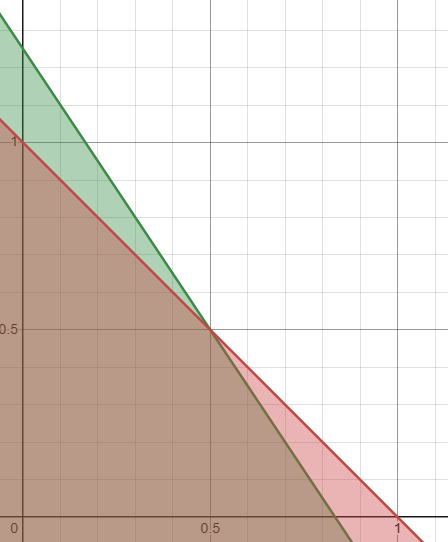
\includegraphics[height=0.8\textheight]{imgs/chvatalgomory.png}

\column{0.6\textwidth}

\only<1>{
\begin{itemize}
\item  $\min_{x,y} -y$\\$\text{s.t. }\frac{3}{2}x + y \leq \frac{5}{4}, (x,y) \in \mathbb{Z}_{\geq 0}^2$
\item $(x^*,y^*)=(0,1)$
\item $\floor{\frac{3}{2}} \cdot 0 + \floor{1} \cdot 1 = 1 \leq \floor{\frac{5}{4}}$ \cmark
\end{itemize}
}

\only<2>{
\begin{itemize}
\item  $\min_{x,y} -y $\\$\text{s.t. }\frac{3}{2}x + y \leq \frac{5}{4}, (x,y) \in \mathbb{Z}_{\geq 0} \times \mathbb{R}_{\geq 0}$
\item $(x^*,y^*)=(0,\frac{5}{4})$
\item $\floor{\frac{3}{2}} \cdot 0 + \floor{1} \cdot \frac{5}{4} = \frac{5}{4} > \floor{\frac{5}{4}}$ \xmark
\end{itemize}
}

\end{columns}
\end{frame}

\begin{frame}{Basic Mixed Integer Rounding Inequalities I}
\only<1>{
Let $x \in \mathbb{Z}_{\geq 0}, y \in \mathbb{R}_{\geq 0}, b \in \mathbb{R}_{>0} \setminus \mathbb{Z}$. Then
\begin{equation}
x \leq \floor{b} \text{ is a valid inequality for } \{x+y \leq b\}
\end{equation}
and
\begin{equation}
x \geq \ceil{b} \text{ is a valid inequality for } \{-x+y \leq -b\}
\end{equation}
}

\only<2>{
%TODO :  Illustration and math proof
}
\end{frame}

\begin{frame}{Basic Mixed Integer Rounding Inequalities II}
\only<1>{
Let $x \in \mathbb{Z}_{\geq 0}, y \in \mathbb{R}_{\geq 0}, b \in \mathbb{R}_{>0} \setminus \mathbb{Z}$. Then
\begin{equation}
x - \frac{1}{f_b-1} \leq \floor{b} \text{ is a valid inequality for } \{x-y \leq b\}
\end{equation}
and
\begin{equation}
x + \frac{1}{f_b} \geq \ceil{b} \text{ is a valid inequality for } \{-x-y \leq -b\}
\end{equation}
}

\only<2>{
%TODO :  Illustration and math proof
}

\end{frame}

\begin{frame}{General Mixed Integer Rounding Inequality}

\only<1>{
Let $F_{MIR} = \{(x,y) \in \mathbb{Z}_{\geq 0}^2 \times \mathbb{R}_{\geq 0} \:\vert\: a_1x_1+a_2x2-y\leq b \}$ where $a \in \mathbb{R}^2, b \in \mathbb{R} \setminus \mathbb{Z}$ and assume that $f_1 \leq f_b \leq f_2$. Then the inequality

\begin{equation*}
\floor{a_1}x_1 + \left( \floor{a_2}+ \frac{f_2 - f_b}{1 - f_b} \right) x_2 - \frac{1}{1-f_b}y \leq \floor{b}
\end{equation*}
is valid for $F_{MIR}$.
}

\only<2>{
%TODO Math Proof
}

\end{frame}

\begin{frame}{Simplex Algorithm}
Simplex finds $\hat{x} \in P \times \mathbb{R}_{\geq 0}^{N-n}$ and creates the optimal simplex tableau:
\begin{center}
\begin{minipage}{0.8\textwidth}
	\begin{tcolorbox}[colback=white, title={$i-$th row in the simplex tableau}]
    \begin{equation*}
    	x_{B_i} + \sum\limits_{\substack{j \in NB}} \bar{a}_{ij} x_j = \bar{b_i}
    \end{equation*}
    \end{tcolorbox}
\end{minipage}
\end{center}
\begin{columns}
\column{0.5\textwidth}
\begin{itemize}
\item $x_1,...,x_{n_1}$: Integral decision variables
\item $x_{n_1+1},...,x_n$: Real decision variables
\item $x_{n+1},...,x_N$: (Real) slack variables
\end{itemize}

\column{0.5\textwidth}
\begin{itemize}
\item $B=\{B_1,...,B_m\}$: Basic variables
\item $NB = \{1,...,N\} \setminus B$: Nonbasic variables ($\hat{x}_j=0$ for $j \in NB$)
\end{itemize}
\end{columns}
%Note: In some cases we also know that some slack variables must be integer
\end{frame}

\begin{frame}{Gomory Mixed Integer Cut}

\only<1>{
Let $N_1= NB \cap \{1,...,n_1\}, N_2 = NB \cap \{n_1+1,...,N\}$. Consider the $i-$th row in the optimal simplex tableau
\begin{equation*}
    x_{B_i} + \sum\limits_{\substack{j \in N_1}} \bar{a}_{ij} x_j + \sum\limits_{\substack{j \in N_2}} \bar{a}_{ij} x_j = \bar{b_i}
\end{equation*}
and assume $B_i \leq n_1$ but $\hat{x}_{B_i}=\bar{b_i} \notin \mathbb{Z}$. Then the \emph{Gomory Mixed Integer Cut}
\begin{tcolorbox}[colback=white]
\begin{equation*}
x_{B_i} + \sum\limits_{\substack{j \in N_1 \\ f_{ij} \leq f_i}} \floor{\bar{a}_{ij}} x_j + \sum\limits_{\substack{j \in N_1 \\ f_{ij} > f_i}} \left( \floor{\bar{a}_{ij}} + \frac{f_{ij}-f_i}{1-f_i} \right) x_j + \sum\limits_{\substack{j \in N_2 \\ \bar{a}_{ij} < 0}} \left( \frac{\bar{a}_{ij}}{1-f_i} \right) x_j \leq \floor{\bar{b_i}}
\end{equation*}
\end{tcolorbox}
% Remark: In literature often with four sums and ... >= f_b. One is obtained by subtracting the other from the initial row.
% Math Proof

is a valid inequality for $F$ that is not satisfied by $\hat{x}$.
}

\only<2>{
%TODO Proof
}

\end{frame}

\begin{frame}{Cutting Planes Algorithm}
\begin{itemize}
\item Let a MILP be given with feasible region $F = \{x \in \mathbb{Z}_{\geq 0}^{n_1} \times \mathbb{R}_{\geq 0}^{n-n_1} \:\vert\: Ax \leq b \}$ for some $A \in \mathbb{R}^{m \times n}, b \in \mathbb{R}^m$.
\item The relaxation is the LP obtained by removing the integer constraints, so its feasible region is the polyhedron $P = \{x \in \mathbb{R}_{\geq 0}^{n} \:\vert\: Ax \leq b \}$.
\item Repeat the following two steps until $\hat{x} \in F$:
\begin{enumerate}
\item Solve the LP using the Simplex Algorithm and obtain $\hat{x} \in P$
\item If the problem is infeasible ($P = \emptyset$), return INEASIBLE. If the problem is unbounded and no integer constraints are violated, return UNBOUNDED
\item If $\hat{x} \notin F$, pick $i \in \{1,...,n_1\}$ s.t. $\hat{x}_i \notin \mathbb{Z}$ and add the corresponding GMI-Cut to the LP.
\end{enumerate}
\end{itemize}
\end{frame}

\begin{frame}{Project Demonstration}
\begin{itemize}
\item Simplex Solver
\item Mixed Integer Gomory Cut
\item 2D Visualisation
\end{itemize}

%\begin{tcolorbox}[colback=white, title={MILP Standard Form}]
%    \begin{align*}
%    	\min_{x}\quad &-y \\
%    	\text{s.t.}\quad & 3x + 2y \leq 6 \\
%    	& -3x + 2y \leq 0 \\
%    	& x, y \in \mathbb{Z}_{\geq 0}
%    \end{align*}
%    \end{tcolorbox}
%    
%    %Also mention resubstitution of slack variables
\end{frame}

\begin{frame}{Cutting Planes Selection}
\begin{itemize}[<+->]
\item Only adding an arbitrary, single cutting plane is very inefficient if the problem dimension is large.
\begin{itemize}
\item Evaluate the efficiency of a cutting plane based on some heuristics (for example euclidean distance to $\hat{x}$).
\item Add multiple cutting planes in each iteration.
\end{itemize}
\item Other cutting plane strategies exist:
\begin{itemize}
\item Knapsack Covers or GUB (generalized upper bound) covers for binary programs.
\end{itemize}
\end{itemize}
\end{frame}

% See AOPT
\section{Branch \& Bound}

\begin{frame}{Branch \& Bound}
\begin{itemize}
\item Like Cutting Planes, we solve the problem relaxation and add constraints until an optimal solution has been found.
\item Divide \& Conquer
\end{itemize}
\end{frame}

\begin{frame}{Branching}
Cut off the non-integer neighborhood of $x_i^* \notin \mathbb{Z} \Rightarrow \text{ Two new relaxation problems}$
\end{frame}

\begin{frame}{Bounding}
\begin{itemize}
\item Initially, we only know that $-\infty < c^\top x_{MILP}^* < \infty$ (not very helpful).
\item Improve bounds until Upper Bound $-$ Lower Bound $< \epsilon$:
\begin{itemize}
\item Lower Bound: For any LP-Relaxation, we have $c^\top x_{LP}^* \leq c^\top x_{MILP}^*$
\item Upper Bound: By definition, $c^\top x_{MILP}^* \leq c^\top x$ for any feasible $x \in F_{MILP}$
\end{itemize}

\end{itemize}
\end{frame}

\begin{frame}{Cutting Planes + Branch \& Bound = Branch \& Cut }
\begin{itemize}
\item Used by many commercial solvers %TODO reference, examples
\item Branch \& Bound but add cuts before branching.
\end{itemize}
\end{frame}

\section{Outro}

\begin{frame}{Questions?}
%TODO Some graphics of the presentation (like in HexEx slides)
\end{frame}

\begin{frame}{References}
    \printbibliography
\end{frame}
 
\end{document}